\documentclass{article}
\usepackage{amsmath}
\usepackage{graphicx}
\usepackage{hyperref}
\title{Investing notes}
\date{10-19-2022}
\author{Tommy Bui}

\begin{document}
	\maketitle
	\newpage
	\pagenumbering{arabic}

	\tableofcontents
	\newpage

	\section{Analyzing a stock from Yahoo Finance} 
	
	\begin{figure}[h!]
		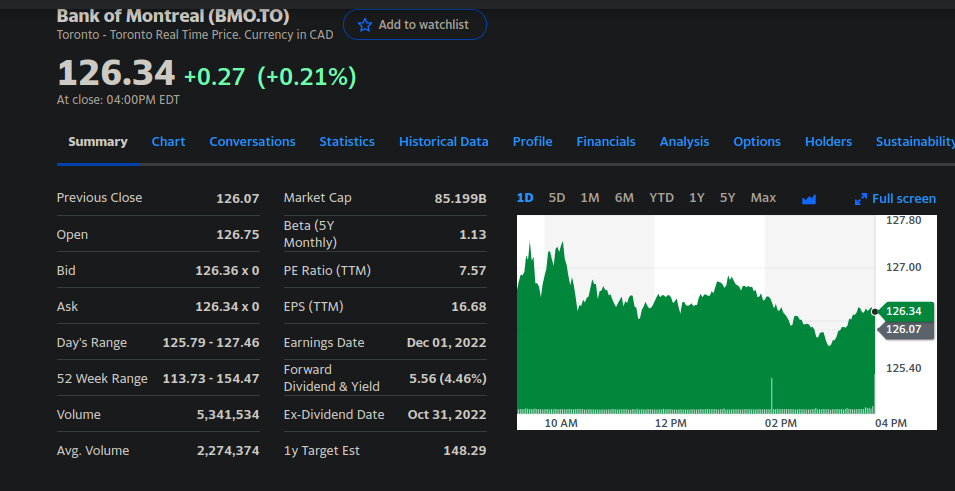
\includegraphics[width=\linewidth]{InvestingPics/figure1.png}
		\caption{View of \$BMO.TO in Yahoo Finance}
		\label{fig:chart1}
	\end{figure}

	%Figure \ref{fig:chart1} is a chart of BMO.TO

	\subsection{Analyzing the Summary Tab}

	\begin{itemize}
		\item {\bf Previous Close:} represents the last closing price reported of a security during a given time period; A security's previous close is an important value that is used by investors to chart gap patterns which can show substantial changes from a previous close to a new open.
		\item {\bf Open:} AKA the opening price; this is the value that a security is initially valued when the exchange opens for the day.
		\item {\bf Bid:} AKA the bidding price; A bid is an offer made by an investor, trader, or dealer in an effort to buy an asset or compete for a contract; The spread between the bid and asking price is a reliable indicator of supply \& demand for the security.
		\item {\bf Ask:} AKA asking price; The price at which someone is willing to sell a security for.
		\item {\bf Range:} Refers to the difference between the highest \& lowest prices a security or index ranges over an interval of time.
		\item {\bf Volume:} Trading volume is a measure of how much a given asset has been traded over a period of time. For stocks, volume is measured in the number of shares traded, for futures \& options, volume is based on how many contracts have changed hands. Volume can indicate market strength, as rising markets on increasing volume are typically viewed as strong and healthy.
		\item {\bf Avg. Volume:}
		\item {\bf Market Cap:} Market capitalization is calculated by multiplying the number of shares outstanding by the current price of a single share (i.e. A company with 50 mil shares \& a stock price \$100 per share would have a market cap of \$5 bil). Market cap is a metric based on stock price. \underline{Market capitalization is used to help define the value of a company when analyzing potential trade opportunities}. 
		\item {\bf Beta (5Y monthly):} Beta measures how volatile a stock is in relation to the broader stock market over the last 5 years, using one data point per month. A stock with a high beta indicates it's more volatile than the overall market and can react with dramatic share-price changes amid market swings. 
			\begin{itemize}
				\item A beta of one means that an investment is as volative as the rest of the market. If the security has a beta of two, it means that the stock is twice as volatile as the market. 
				\item Low risk traders often avoid investing in high-beta stocks.
				\item Beta relies on past information and so doesn't help describe the fundamentals of the security, however a beta may be a strong factor in quantifying risk for frequent traders
			\end{itemize}
		\item {\bf \hyperref[sec:PER]{Price-to-Earnings (P/E) Ratio}:} The price-to-earnings (P/E) ratio relates a company's share price to its earnings per share.
		\item {\bf Earnings Per Share (EPS):} Calculated as a company's profit divided by the outstanding shares of its common stock. The resulting number is an measure of the company's profitability. A higher EPS indicates greater value since investors will pay more for a company's shares if they believe the company has higher profits relative to its share price.
		\item {\bf Earnings Date:} This is the date when a company will annouce its financial position, companies in the public sector typically do this every quarter. Traders often take into account the next earnings date as the share price often fluctuates around this time period; If a company has been profitable leading up to the annoucment, its share price will usually increase up to \& slightly after the info is released. 
		\item {\bf Forward Dividend \& Yield:} Measures the estimated yearly dividend; The first part of the metric is the year's projected dividend and is calculated by taking a stock's most recent actual dividend payment \& annualizing it. The second part of the metric is the percentage of a company's current stock price that it expects to pay out as dividends over a year. It is calculated by dividing a year's worth of future divident payments by a stock's current share price \& is represented as a percentage.
			\begin{itemize}
				\item This metric is used to estimate the divident for the next year. It is most useful when the yield is predictable based on past instances. If this is not the case, trailing yields can be used, which indicate the same value over the previous 12 months.
			\end{itemize}
		\item {\bf Ex-divident date (ex-date):} is one of four stages that companies go through when they pay dividends to their shareholders. The ex-dividend date determines whether the investor is eligible to recieve its upcoming dividend; Consider the ex-dividend date as the cutoff point for shareholders to be credited a pending stock dividend.
		\item {\bf 1y Target Est:} One year target estimate is the projected price of the security in one year's time. It is based on analyst's estimates after considering numerous fundamental and techincal factors. {\bf Note:} This is still a guess.
	\end{itemize}
	
	\section{P/E Ratio}
	\label{sec:PER}

		\subsubsection{Overview}
		\begin{itemize}
		\item The ratio represents the factor which traders are willing to buy the security (price) compared to the profit gained by the company (EPS) with the sale of the security.
			\item A high (P/E) ratio could mean that a company's stock is overvalued OR that investors are expecting high growth rates in the future.
			\item According to investopedia, {\bf a P/E ratio holds the most value to an analyst when compared against similar companies in the same industry or for a single company across a period of time.}
			\item In essence, {\bf the P/E ratio indicates the dollar amount an investor can expect to invest in a company in order to receive \$1 of that company's earnings.}
			\item This is why P/E is sometimes referred to as the price multiple since it shows how much investors are willing to pay in dollar amounts per dollar of earnings of that security; If a company was trading at a P/E multiple of 20x, the interpretation is that an investor is willing to pay \$20 for \$1 of that security's current earnings.
			\item {\bf NOTE:} Valuation ratios compare the company's market value with some financial aspect of its performance - earnings, sales, book value, cash flow, and so forth; the ratio-based approach is the most commonly used method for valuing stocks since ratios are easy to calculate and readily available. The downside of making sense of valuatio ratios is that they require a quite a bit of context (i.e. A P/E ratio of 15 does not mean much unless you know the P/E of the market as a whole, the P/E's of the company's main competitors, the company's historical P/E's, and similar information.
			\item These two types of EPS metrics factor into the most common P/E ratios: the {\bf forward P/E} and the {\bf trailing P/E}.
			\item The forward (or leading) P/E uses future earnings guidance rather than trailing figures. Sometimes called "Estimated price to earnings", this
				forward indicated is useful for comparing current earnings to future earnings and helps provided a clear picture of what earnings will look like.
			\item The main issue with forward P/E metric is that companies could underestimate earnings in order to beat the estimate P/E or may overstate the estimate and later adjust it going into their next earnings annooucement.
			\item Trailing Price-to-Earnings relies on past performance by dividng the current share price bye the total EPS earnings over the past 12 months; it's the most popular P/E metric because its the most objective (assuming companies reported their earnings accurately)
			\item The trailing P/E has its share of shortcomings as well, namely, that a company's past performance doesn't reflect future behavior; thus investors should commit money based on future earnings power, not the past.
			\item If an EPS remains constant, while the stock pricecs fluctuate, is a problem. If a major company event drives the stock prices higher or lower, the trailing P/E will be less reflective of those changes.
			\item If the forward P/E is lower than the trailing P/E, it means analyst expect earnings to increase; if the foward P/E is higher than the current P/E, analysts expect them to decrease
			\begin{align*}
				Price-to-Earnings (P/E) ratio &= \frac{Market Value Per Share}{Earnings Per Share}\\
			\end{align*}
			\item Consider this example where we compare two financial company's P/E ratio to determine which is over/undervalued:
				\begin{itemize}
					\item Bank of America Corporation \$BAC closed out the 2020 year with the following:
						\begin{itemize}
							\item {\bf Stock Price} = \$30.31
							\item {\bf Diluted EPS} = \$1.87
							\item ${\bf P/E} = 16.21 = (\$30.31/\$1.87)$
						\end{itemize}
					\item In short, \$BAC was traded at roughly 16 times its trailing earnings. However, the 16.21 P/E multiple by itself is not helpful unless you have something to compare it to. Lets compare \$BAC with JPMorgan Chase \& Co. (\$JPM) of 2020:
						\begin{itemize}
							\item {\bf Stock Price} = \$127.07
							\item {\bf Diluted EPS} = \$8.88
							\item {\bf P/E} = 14.31x
						\end{itemize}
					\item When you compare \$BAC's P/E of 16x to \$JPM's P/E of roughly 14x, \$BAC's stock does not appear as overvalued as it did compared with the average P/E of 15 for the S\&P 500. \$BAC's higher P/E ratio might mean investors expected higher earnings growth in the future compared to \$JPM and the overall market.
					\item However, no single ratio can tell you all you need to know about a stock. \underline{Before investing, it is wise to use a variety of financial ratios to determine whether a stock 
						is fairly valued and whether a company's financial health justifies its stock valuation}.
					\item In general, a high P/E suggests either investors are expecting higher earnings growth in the future compared to companies with a lower P/E {\bf OR} the security is overvalued.
					\item A low P/E can indicate either that a company may currently be undervalued or that the company is doing exceptionally well relative to its past trends.
					\item When a company has no earnings ot is posting losses, {\bf the P/E will be expressed as N/A}. 
					\item The P/E ratio can be seen as a means of standardizing the value of a \$1 of earnings throughout the stock market. In theory, by taking the median of P/E ratios over a period of several years, one could formulate something of a standardized P/E ratio, which could then be seen as a benchmark and used to indicated whether or not a stock is worth buying. 
					\item The inverse of P/E ratio is the earnings yield (E/P ratio) which is defined as EPS per \$ value of the stocks price expressed as a percentage; but this metric is not widely used compared to P/E ratio.
					\item Earnings yield may be useful when concerned about the rate of return on investment.
					\item {\bf Limitations of Using the P/E Ratio:}
						\begin{itemize}
							\item A P/E ratio, even one calculated using a forward earnings estimate, doesn't always tell you whether the P/E is appropiate for teh company's forecasted growth rate. So Investors may look into another ratio called the \underline{PEG Ratio} (Profit-to-Earnings-Growth).
						\end{itemize}

					\item A variation on the forward P/E ratio is the \underline{price/earnings-to-growth ratio} or PEG. The PEG ratio measures the relationship between the price/earnings ratio \& earnings growth to provide investors with more details. In other ways, the PEG ratio allows investors to calculate whether an equity is overvalued or undervalude by analyzing both today's earnings \& the expected growth rate for the company in the future. The PEG ratio is calculated as a company's trailing price-to-earnings (P/E) ratio divided by the growth rate of its earnings for a specific time.
				\end{itemize}
		\end{itemize}
	{\bf Is It Better to Have a Higher or Lower P/E Ratio?} \newline

	Many investors will say that companies with a lower P/E are more valuable as you are paying less money for reach dollar of earnings that equity receives. In this regard, a lower P/E is like a lower price tag, making it attractive to investors looking for a bargain. In practice it is important to understand the reasons behind a company's P/E. For instance, if a company has a low P/E because its business model is fundamentally in decline, then the apparent bargain might be an illusion.

	\subsubsection{Earnings Estimate}



	\section{Fundamental Analysis}
	\url{https://www.investopedia.com/terms/f/fundamentalanalysis.asp} \newline
	\url{https://www.investopedia.com/articles/trading/06/fundamentalapproach.asp}

	\subsection{Overview}

	Fundamental Analysis is a method ussd to determine the true value of a security. Fundemental Analysis (FA) measures a \href{https://www.investopedia.com/terms/v/valuation.asp}{a security's intrinisic value}
	by examining related economic \& financial factors. Intrinsic value is the value of an investment based on the issuing company's financial situation \& current market \& economic conditions.
	Fundamental analysts study anything that can affect the security's value, from macroeconomic factors such as the state of the economy \& industry conditions to microeconomic factors like the 
	effectiveness of the company's management. \newline

	Key Takeaways:
	\begin{itemize}
		\item The end goal is to determine whether the security's current price is either undervalued or overvalued by other investors. Fundamental analysis is a method of determining a stock's real/fair value.
		\item If the fair market value is higher than the market price, the stock is deemed undervalued, thus it may be recommended to buy the security.
		\item If the fair market value is lower than the market price, the stock is deemed overvalued, thus it may be recommened to either hold, sell, or stop buying the stock.
		\item In constrast, technical analysts favor studying the historical price trends of the stock to predict short-term future trends.
	\end{itemize}
	
	\subsection{Understanding Fundamental Analysis}
	Fundamental analysis is take from a macro-to-micro perspective to identify the true value of securities in the market. Fundamental analysis in layman term's tells you the true
	price of a security. \newline

	Analysts typically study, in order:
	\begin{itemize}
		\item The overall state of the economy
		\item The strength of the specific industry
		\item The financial performance of the company issuing the stock
	\end{itemize}

	This ensures analysts arrive at a fair market value for the stock.

	\subsection{Sources for Fundamental Analysis}

	Fundamental analysis uses publicly available financial data to evaluate the value of a security. The data is recorded on financial statements such as quarterly \&
	annual reports \& filings like the 10-Q (quarterly) or 10-K (annual). The 8-K is also informative because public companies must file it anytime a reportable event occurs, like an 
	acquisition or upper-level management change.	\newline
	
	{\bf NOTE:} Most public-and many private companies list annual reports on the investor relation sections of their websites, which highlight financial decisions made \& results achieved 
	throughout the year. \newline

	For example, you may perform a fundamental analysis of a bond's value by examining economic factors such as interest rates \& the overall state of the economy.
	Then you would evaluate the bond market \& use financial data from similar bond issuers. Finally you'd analyze the financial performance of the bond by examining the finacial data from the issuing
	compny, including external factors such as potential changes in its \href{https://www.investopedia.com/terms/c/creditrating.asp}{credit rating}. You would also read through the 8-K, 10-Q, 10-K,
	\& the issuer's annual reports to find out what they are doing, their objectives, their weakness, etc. \newline

	Fundamental analysis uses a company's revenues, earnings, future growth, \href{https://www.investopedia.com/terms/r/returnonequity.asp}{return on equity}, profit margins, and other data to
	determine a company's underlying value \& potential for future growth.

	\subsection{Intrinsic value}

	The primary assumptions behind fundamental analysis is that a stock's current price does not accurately reflect the value of the compnay when compared to publicly available financial data. A
	second assumption is that the value reflected from the company's fundamental data is more likely to be closer to the true value of the stock. \newline

	Fact: The term, \textit{intrinsic value} means something different in stock valuation compared to options trading. Option pricing uses a standard calculation for intrinsic value, while it can
	be calculated in many different ways for a stock. \newline

	Consider if a company's stock was traded \@ \$20, and after extensive research on the company, an analyst determines that it ought to be worth \$24. Meanwhile, another analyst also researchs the same
	company and determines that the security should be worth \$26. \newline

	Many investors will consider the average of these estimates and assume that the stock's intrinsic value may be near \$25. Ofter investors consider these estimates highly relevant since they want to
	by stocks that are being traded significantly below these intrinsic values. \newline

	This leads to a third major assumpmtion of fundamental analysis: \textit{ {\bf In the long run, the stock market will reflect the fundamentals}. The problem is, no one knows how long "the long run"
	really is. It could be days or years}. \newline

	This is the main concept of fundamental analysis. By focusing on a particular business, an investor can estimate the intrinsic value of a firm \& find opportunities to buy at a discount or sell 
	at a premium.  {\bf The investment will pay off when the market catches up to the fundamentals.} \newline

	\subsection{Fundamental Analysis vs. Technical Analysis}

	This method of analysis starkly constrasts with \href{https://www.investopedia.com/terms/t/technicalanalysis.asp}{technical analysis}, which attempts to forecast the trend through analyzing
	historical market data such as {\bf price} \& {\bf volume}. Technical analysis uses the trends \& actions in the price of the security to create indicators. Some of the indicators create 
	patterns that have names resembling their shapes, such as the head \& shoulders pattern. Others use trend, support, \& resistance lines to demonstrate how traders view investments \& indicate what
	will happen. Some examples are the symmetrical triangle or the wedge. \newline

	Fundamental analysis relies on financial information reported by the company whose stock is being analyzed. Ratios \& metrics are created using the data which indicates how a company is performing
	compared to companies in the same industry.

	\subsection{Quantitative \& Qualitative Fundamental Analysis}

	The problem with defining the word fundamentals is that it can cover anything related to the economic well-being of a company. They include numbers like revenue \& profit, but they can also 
	include numbers like revenue \& profit, but they can also include anything from a company's market share to the quality of its management. \newline

	The various fundamental factors can be grouped into two categories: quantitative \& qualitative. The financial meaning of these terms isn't much different from well-known definitions: \newline

	\begin{itemize}
		\item {\bf Quantitative:} information that can be shown using numbers, figures, ratios, or formulas
		\item {\bf Qualitative:} rather than a quantity of something, it is its quality, standard, or nature
	\end{itemize}

	In this context, quantitative fundamentals are a measurable characteristic of a business. Thus the biggest source of quantitative data is financial statements. Revenue, profit, assets, \& more
	can be accurately measured. \newline

	Qualitative fundamentals involve non-tangible characteristics. They might include the quality of a company's key executives, brand-name recognition, \href{https://www.investopedia.com/terms/p/patent.asp}{patents},
	and \href{https://www.investopedia.com/terms/p/proprietarytechnology.asp}{proprietary technology}. \newline

	Neither qualitative nor quantitative analaysis is inherently better. Many analysts consider them equal. \newline

	\subsection{Qualitative Fundamentals to Consider}

	There are four key fundamentals that analysts always consider when regarding a company. \underline{All are qualitative rather than quantitative.} They include:

	\subsubsection{The Business Model}

	What exactly does the company do? This isn't as straightforward as it seems. If a company's business model is based on selling fast-food chicken, is it making its money that way? Or is it just
	coasting on royalty \& franchies fees?

	\subsubsection{Competitive Advantage}

	A company's long-term sucess is primarily driven by its ability to maintain a competitive advantage-and keep it. Powerful competitive advantages, such as Coca-Cola's brand name \& Microsoft's
	domination of the personal computing operating system, create a \href{https://www.investopedia.com/ask/answers/05/economicmoat.asp}{moat} around a business allowing it to keep competitors at bay
	\& enjoy growth \& profits. When a company can achieve a competitive advantage, its shareholders can be well rewarded for decades. \newline

	\subsubsection{Management}

	Some believe management is the most important criterion for investing in a company. It makes sense: Even the best business model is doomed if the company's leaders fail to execute the plan
	properly. While it's hard for retail investors to meet \& truly evaluate managers, you can look at the corporate website and {\bf check the resumes of the top brass \& the board members}. How
	well did they perform it previous jobs? Have they have been unloading a lot of their stock shares lately? \newline

	\subsubsection{Corporate Governance}

\end{document}
